\chapter[Grundlagen]{Grundlagen}
\label{chap:definitions}

In diesem Kapitel werden theoretische Grundlagen, die für die Arbeit relevant sind erläutert. Hier sind einige Beispiele für Latex Inhalte, wie Zitate, Abbildungen, Listen und Tabellen.

\section{Abbildungen}

\begin{figure}[h]
    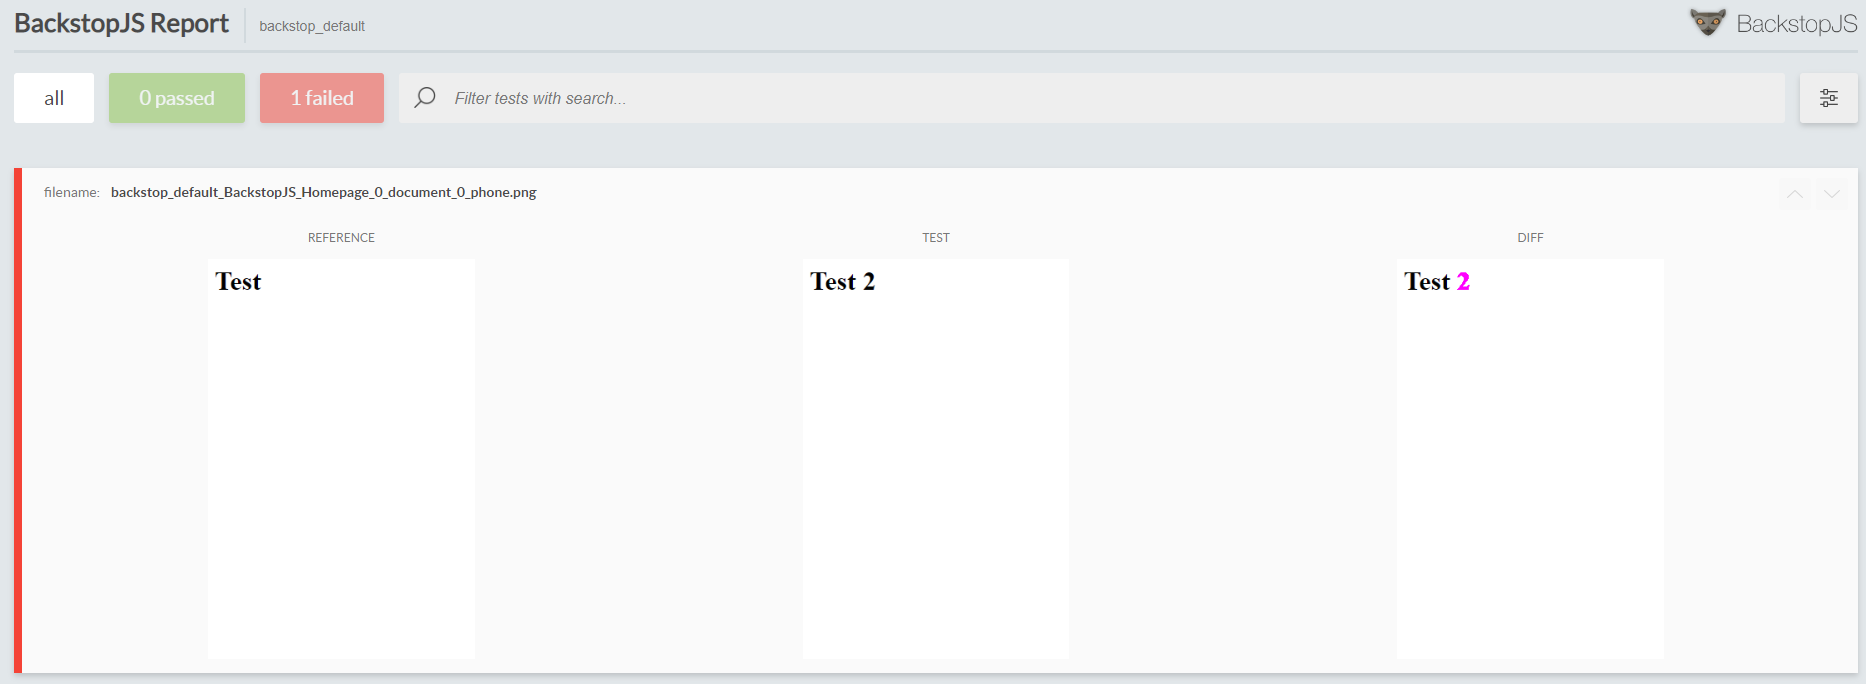
\includegraphics[width=1\linewidth]{src/Backstop.png}
    \centering
    \captionbelow[Screenshot aus BackstopJS]{Screenshot aus BackstopJS (eigene Darstellung)}
    \label{fig:backstopjs}
\end{figure}

\begin{landscape}
    \begin{figure}[h]
        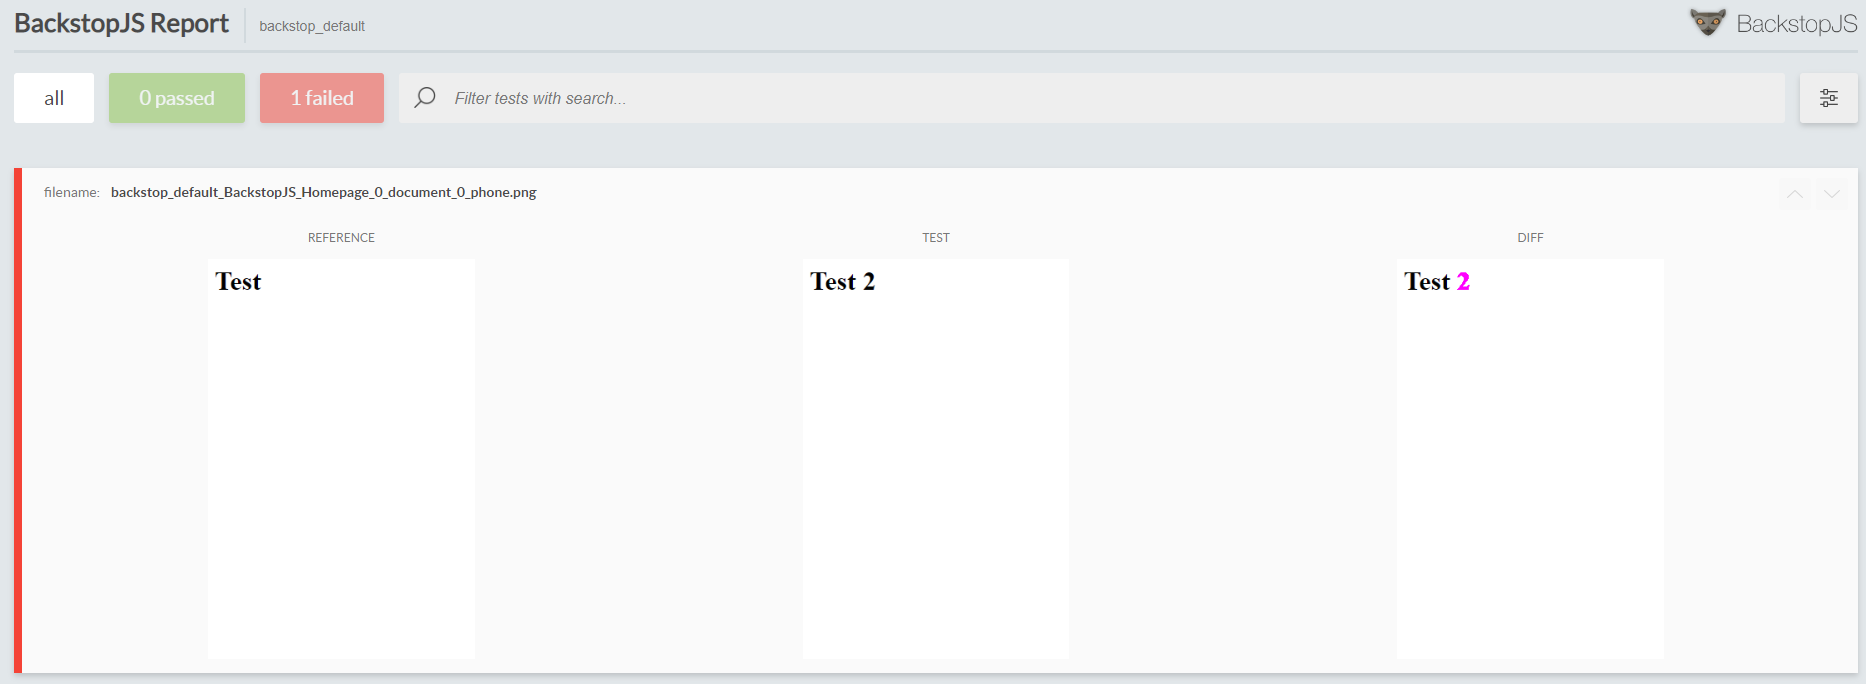
\includegraphics[width=1\linewidth]{src/Backstop.png}
        \centering
        \captionbelow[Screenshot aus BackstopJS im Querformat]{Screenshot aus BackstopJS im Querformat(eigene Darstellung)}
        \label{fig:landscape-backstopjs}
    \end{figure}
\end{landscape}

\section{Tabellen}
\begin{table}[h]
    \centering
    \renewcommand*{\arraystretch}{1.5}
    \begin{tabular}{|l|l|l|}
        \hline
               & Achsen & Räder \\ \hline
        Auto   & 2      & 4     \\ \hline
        Moped  & 2~     & 2~    \\ \hline\hline
        Gesamt & 4      & 6     \\ \hline
    \end{tabular}
    \captionbelow{Mehr oder weniger sinnvolle Tabelle}
    \label{tab:example-table}
\end{table}

\section{Zitate}

\subsection{Direktes Zitat}
\begin{quote}
    \glqq Hier könnte Ihre Werbung stehen.\grqq
    \begin{flushright}
        Musterwerbefirma~\cite{web}
    \end{flushright}
\end{quote}

\subsection{Indirektes Zitat}
Bei Büchern sollte immer eine Seitenzahl angegeben werden. \cite[S.~1]{book}

\section{Auflistungen}

\subsection{Einfache Auflistung}
\begin{itemize}
    \item Punkt 1
    \item Punkt 2
\end{itemize}

\subsection{Auflistung mit Beschreibung}
\begin{description}
    \item[Punkt 1:]
        Beschreibung

    \item[Punkt 2:]
        Beschreibung
\end{description}

\section{Referenzierung}
Referenzierungen können auf alle Label vorgenommen werden, wie Abbildungen (\autoref{fig:backstopjs}), Tabellen (\autoref{tab:example-table}), Kapitel (\autoref{chap:introduction}) oder auch auf die Seitenzahl eines Labels (Seite \pageref{fig:backstopjs}).